\begin{enumerate}[label=\thechapter.\arabic*,ref=\thechapter.\theenumi]

\item The number of zeroes of the polynomial $P(s) = s^3+2s^2+5s+80$ in the right side of the plane?\hfill(GATE IN 2023) \\

\solution
% \iffalse
\let\negmedspace\undefined
\let\negthickspace\undefined
\documentclass[journal,12pt,twocolumn]{IEEEtran}
\usepackage{cite}
\usepackage{amsmath,amssymb,amsfonts,amsthm}
\usepackage{algorithmic}
\usepackage{graphicx}
\usepackage{textcomp}
\usepackage{xcolor}
\usepackage{txfonts}
\usepackage{listings}
\usepackage{enumitem}
\usepackage{mathtools}
\usepackage{gensymb}
\usepackage{comment}
\usepackage[breaklinks=true]{hyperref}
\usepackage{tkz-euclide} 
\usepackage{listings}
\usepackage{gvv}                                        
\def\inputGnumericTable{}                                 
\usepackage[latin1]{inputenc}                                
\usepackage{color}                                            
\usepackage{array}                                            
\usepackage{longtable}                                       
\usepackage{calc}                                             
\usepackage{multirow}                                         
\usepackage{hhline}                                           
\usepackage{ifthen}                                           
\usepackage{lscape}
\newtheorem{theorem}{Theorem}[section]
\newtheorem{problem}{Problem}
\newtheorem{proposition}{Proposition}[section]
\newtheorem{lemma}{Lemma}[section]
\newtheorem{corollary}[theorem]{Corollary}
\newtheorem{example}{Example}[section]
\newtheorem{definition}[problem]{Definition}
\newcommand{\BEQA}{\begin{eqnarray}}
\newcommand{\EEQA}{\end{eqnarray}}
\newcommand{\define}{\stackrel{\triangle}{=}}
\theoremstyle{remark}
\newtheorem{rem}{Remark}
\begin{document}
\parindent 0px

\bibliographystyle{IEEEtran}
\vspace{3cm}

\title{Assignment\\[1ex]GATE-EC-39}
\author{EE23BTECH11034 - Prabhat Kukunuri$^{}$% <-this % stops a space
}
\maketitle
\newpage
\bigskip

\renewcommand{\thefigure}{\theenumi}
\renewcommand{\thetable}{\theenumi}
\section{Question}
Consider the circuit shown in the figure with input V(t) in volts.The sinusoidal steady state current I(t) flowing through the circuit is shown graphically(where t is in seconds). The circuit element Z can be\rule{1.5cm}{0.15mm}.
\begin{enumerate}
    \item a capacitor of 1 F
    \item an inductor of 1 H
    \item a capacitor of $\sqrt{3}$ H
    \item an inductor of $\sqrt{3}$ H
\end{enumerate}
\begin{figure}[ht]
    \centering
    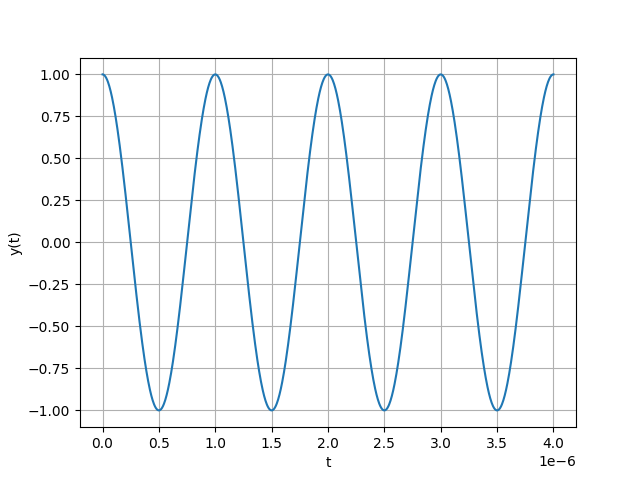
\includegraphics[width=\columnwidth]{figs/Figure_1.png}
    \label{fig:GATE.2022.EC.39.1}
\end{figure}
\solution\\
\begin{table}[h]
    \centering
    \begin{tabular}{|p{2cm}|p{2.80cm}|p{2.70cm}|}
    \hline
    Symbol&Value&Description\\ \hline
    $$x(n)$$&$$(x(0)+nd)u(n)$$&$$n^{th}$$ term of an A.P\\ \hline
    $$x(0)$$&$$x(0)$$&$1^{st}$ term of the A.P\\ \hline
    $$d$$&$$d$$&Common difference\\ \hline
    $$y(n)$$&$$x(n)\ast u(n)$$&Sum of n terms of an AP\\ \hline
    $$a$$&$$y(p-1)$$&Sum of first p terms of the AP\\ \hline
    $$b$$&$$y(q-1)$$&Sum of first q terms of the AP\\ \hline
    $$c$$&$$y(r-1)$$&Sum of first r terms of the AP\\ \hline
\end{tabular}
    \caption{Variable description}
    \label{tab:GATE.2022.EC.39.1}
\end{table}\\
The current through the circuit can be expressed as
\begin{align}
    I(t)=\sin\brak{t-\frac{\pi}{4}}
\end{align}
Since, the voltage seems to be leading the current the circuit element z is an inductor with inductance L.\\
Applying KVL in the circuit,
\begin{align}
    R.I\brak{t}+L\frac{dI\brak{t}}{dt}=sin\brak{t}
\end{align}
Applying Fourier transform to the differential equation,
\begin{align}
    &R.I\brak{s}+sL.I\brak{s}-\frac{1}{s^2+1}=0\\
    &I\brak{s}\brak{R+sL}=\frac{1}{s^2+1}\\
    &\sin\brak{at+b}\system{L}\frac{a\cos\brak{b}+s\sin\brak{b}}{a^{2}+s^{2}}\\
    &\sin\brak{t-\frac{\pi}{4}}\system{L}\frac{1-s}{2\brak{s^2+1}}\\
    &\frac{1-s}{2\brak{s^2+1}}\brak{R+sL}=\frac{1}{s^2+1}
\end{align}
Upon plugging in R=1$\ohm$,
\begin{align}
   L=\frac{1}{s}
\end{align}
Applying inverse Laplace,
\begin{align}
    L=1H
\end{align}

Appendix\\
Laplace transform of $\sin\brak{at+b}$ is as follows,
\begin{align}
    &\sin\brak{at+b}\system{L}\int_{0}^{\infty}\sin\brak{at+b}e^{-st}dt\\
    &\int_{0}^{\infty}\sin\brak{at+b}e^{-st}dt=\cos{b}\int_{0}^{\infty}\sin\brak{at}e^{-st}dt+\sin{b}\int_{0}^{\infty}\cos\brak{at}e^{-st}dt\\
    &\int_{0}^{\infty}\cos\brak{at}e^{-st}dt=\frac{e^{-st}}{a}sin{at}\Bigg|_{0}^{\infty}+\frac{s}{a}\int_{0}^{\infty}\sin\brak{at}e^{-st}dt\\
    &\int_{0}^{\infty}\cos\brak{at}e^{-st}dt=\frac{s}{a}\int_{0}^{\infty}\sin\brak{at}e^{-st}dt\label{eq:GATE.2022.EC.39.2}\\
    &\int_{0}^{\infty}\cos\brak{at}e^{-st}dt=\frac{s}{a}\brak{\frac{-e^{-st}}{a}cos{at}\Bigg|_{0}^{\infty}+\frac{s}{a}\int_{0}^{\infty}\cos\brak{at}e^{-st}dt}\\
    &\int_{0}^{\infty}\cos\brak{at}e^{-st}dt=\frac{s}{a^2}+\frac{s^2}{a^2}\int_{0}^{\infty}\cos\brak{at}e^{-st}dt
\end{align}
\begin{align}
    &\int_{0}^{\infty}\cos\brak{at}e^{-st}dt=\frac{s}{s^2+a^2},s>0
\end{align}
From \eqref{eq:GATE.2022.EC.39.2} we can say,
\begin{align}
    &\int_{0}^{\infty}\sin\brak{at}e^{-st}dt=\frac{a}{s^2+a^2},s>0\\
    &\therefore \sin\brak{at+b}\system{L}\frac{s\sin{b}+a\cos{b}}{s^2+a^2}
\end{align}
\end{document}

\newpage

\item The circuit shown in the figure is initially in the steady state with the switch K in open condition and $\overline{K}$ in closed condition. The switch K is closed and $\overline{K}$ is opened simultaneously at the instant $t = t_1$, where $t_1 > 0$. The minimum value of $t_1$ in milliseconds such that there is no transient in the voltage across the 100 $\mu F$ capacitor, is \rule{1cm}{0.15mm} (Round off to 2 decimal places) \hfill (GATE EE 2023)
    \begin{circuitikz}[american]
        \draw (0,7) to [R=10$\Omega$] (0,2) to [short] (3.5,2) to [isource, l={$\sin\brak{1000t}$}] (3.5,7) to [short] (0,7);
        \draw (3.5,2) to [short] (5,2) to [short] (5,0) to [R=$10\Omega$] (7.5,0) to [battery2 = 5V] (10,0) to [short] (10,2) to [curved capacitor=100$\mu$F, invert] (10,7) to [short] (5,7) to [short] (3.5,7);
        \draw (5,2) to [short] (7, 2) to[ospst=$\overline{K}$] ++(1,0);
        \draw (5,5) to [short] (5,2);
        \draw (10,2) to [short] (8,2);
        \draw (5,7) to [short] (5,6) to[cspst=K] ++(0,-1) ;
\end{circuitikz}


\newpage
\item $y=e^{mx}+e^{-mx}$ is the solution of which differential equation?
\begin{enumerate}[label=\textbf{\arabic*.}, font=\bfseries, align=left]
    \item $\frac{dy}{dx} - my = 0$ 
    \item $\frac{dy}{dx} + my = 0$ 
    \item $\frac{d^{2}y}{dx^{2}} + m^{2}y = 0$ 
    \item $\frac{d^{2}y}{dx^{2}} - m^{2}y = 0$ 
\end{enumerate} \hfill(GATE AG 2023)
\solution

\newpage
\item  A cascade control strategy is shown in the figure below. The transfer function between the output $(y)$ and the secondary disturbance $(d_2)$ is defined as  \\
$$G_{d2}(s)= \frac{y(s)}{d_2(s)}$$. 
Which one of the following is the CORRECT expression for the transfer function $G_{d2}(s)$? \\
\begin{figure}[h]
    \centering
    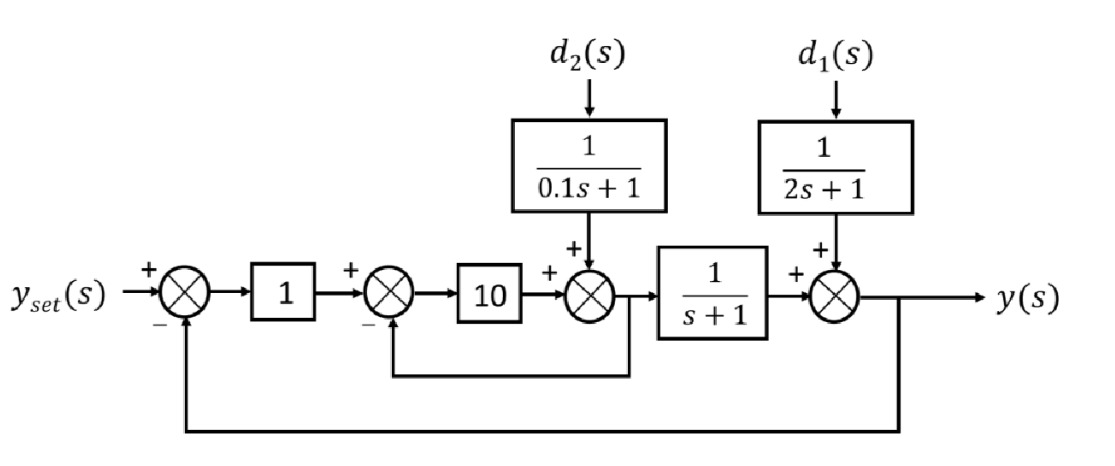
\includegraphics[scale=0.25]{2023/CH/44/figs/g44fig1.jpeg}
    \caption{ }
    \label{}
\end{figure}
\begin{enumerate}[label=\Alph*.]
\item $\frac{1}{(11s+21)(0.1s+1)}$ 
\item $\frac{1}{(s+1)(0.1s+1)}$
\item $\frac{(s+1)}{(s+2)(0.1s+1)}$
\item $\frac{(s+1)}{(s+1)(0.1s+1)}$
\end{enumerate} \hfill (GATE CH 2023)
\solution
\newpage
\item In the differential equation $\frac{dy}{dx} + \alpha x y = 0, \alpha$ is a positive constant. If $y = 1.0$ at
$x = 0.0$, and $y = 0.8$ at $x = 1.0$, the value of $\alpha$ is (rounded off to three decimal places).  \hfill(GATE CE 2023)
\solution
\end{enumerate}
